\documentclass[12pt, border=8pt]{standalone}
\usepackage[table]{xcolor}
\usepackage{tikz}
\usepackage{amsmath, amssymb, bm}
\usepackage{booktabs}
\usetikzlibrary{positioning, arrows.meta, calc, fit, backgrounds, 3d}

% Row alternating colours
\definecolor{rowA}{RGB}{240,246,255}
\definecolor{rowB}{RGB}{255,255,255}

\begin{document}

{\large\itshape Which neural network architecture to use for each problem type}

\vspace{0.5em}

\rowcolors{2}{rowA}{rowB}
\begin{tabular}{p{2.9cm} p{2.4cm} p{3.4cm} p{4.5cm} p{2.4cm}}
\toprule
\rowcolor{gray!18}
\textbf{Task} & \textbf{Input} & \textbf{Architecture} & \textbf{Key Reason} & \textbf{Example} \\
\midrule
Image Classification
  & Image ($H{\times}W{\times}C$)
  & \textbf{CNN}
  & Spatial locality, weight sharing; filters: edges $\to$ shapes $\to$ objects
  & ResNet, EfficientNet \\

Object Detection
  & Image ($H{\times}W{\times}C$)
  & \textbf{CNN + Region Head}
  & Multi-scale feature maps; backbone CNN + detection head
  & YOLO, Faster R-CNN \\

Named Entity Recognition
  & Token sequence
  & \textbf{BiLSTM-CRF / BERT}
  & Bidirectional context per token; CRF models label transitions
  & spaCy, BERT-NER \\

Text Classification
  & Text sequence
  & \textbf{BERT / CNN / LSTM}
  & Global context or local $n$-grams; BERT $\gg$ LSTM $\gg$ CNN accuracy
  & BERT fine-tune \\

Seq-to-Seq
  & Source sequence
  & \textbf{Transformer Enc--Dec}
  & Attention over full source; Encoder reads; decoder attends
  & T5, BART, mT5 \\

Language Modelling
  & Token sequence
  & \textbf{Transformer Decoder (GPT)}
  & Causal left-to-right attention; Masked self-attn: no future tokens
  & GPT-2/3/4, LLaMA \\

Time Series
  & Numeric sequence
  & \textbf{LSTM / Transformer}
  & Temporal state or attention; LSTM moderate; Trans.\ long-range
  & Temporal Fusion Trans. \\

Question Answering
  & [Question, Context]
  & \textbf{BERT + Span Head}
  & Bidirectional understanding; Predicts start/end span in context
  & BERT-large (SQuAD) \\

Semantic Search
  & Text
  & \textbf{Bi-encoder (SBERT)}
  & Dense vector similarity; Encode query \& docs; cosine sim.
  & FAISS, Pinecone \\
\bottomrule
\end{tabular}

\vspace{1.2em}

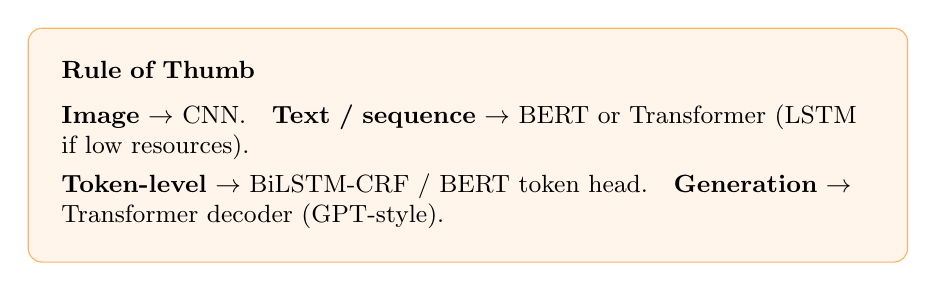
\begin{tikzpicture}
  \node[draw=orange!60, fill=orange!8, rounded corners=5pt,
        inner sep=12pt, text width=\textwidth-1.8cm, align=left, font=\small] at (0,0) {%
    \textbf{Rule of Thumb}\\[5pt]
    \textbf{Image} $\to$ CNN.\quad
    \textbf{Text / sequence} $\to$ BERT or Transformer (LSTM if low resources).\\[3pt]
    \textbf{Token-level} $\to$ BiLSTM-CRF / BERT token head.\quad
    \textbf{Generation} $\to$ Transformer decoder (GPT-style).
  };
\end{tikzpicture}

\end{document}
